\chapter{Sun-BCNN}
\section{Introduction}
A crucial competency of any autonomous mobile robot is the ability to estimate its own motion through an operating environment.
While there exists a rich body of literature on the topic of motion estimation using a variety of techniques such as lidar-based point cloud matching \citep{Zhang2015-gf} and visual-inertial odometry \citep{Leutenegger2015-fk}, egomotion estimation is fundamentally a process of dead-reckoning and will accumulate unbounded error over time.
This accumulated error, or drift, can be limited by incorporating global information into the motion estimation problem.
This frequently takes the form of a globally consistent map, loop closure detection, or reliance on additional sensors such as GPS to make corrections to the estimated trajectory.
In many situations, however, a globally consistent map may be unavailable or prohibitively expensive to compute, loop closures may not occur, or GPS may be unavailable or inaccurate.
In such cases, it can be advantageous to rely on environmental cues such as the sun, which can easily provide global orientation information since it is readily detectable and its apparent motion in the sky is well described by ephemeris models.

\begin{figure}
    \centering
      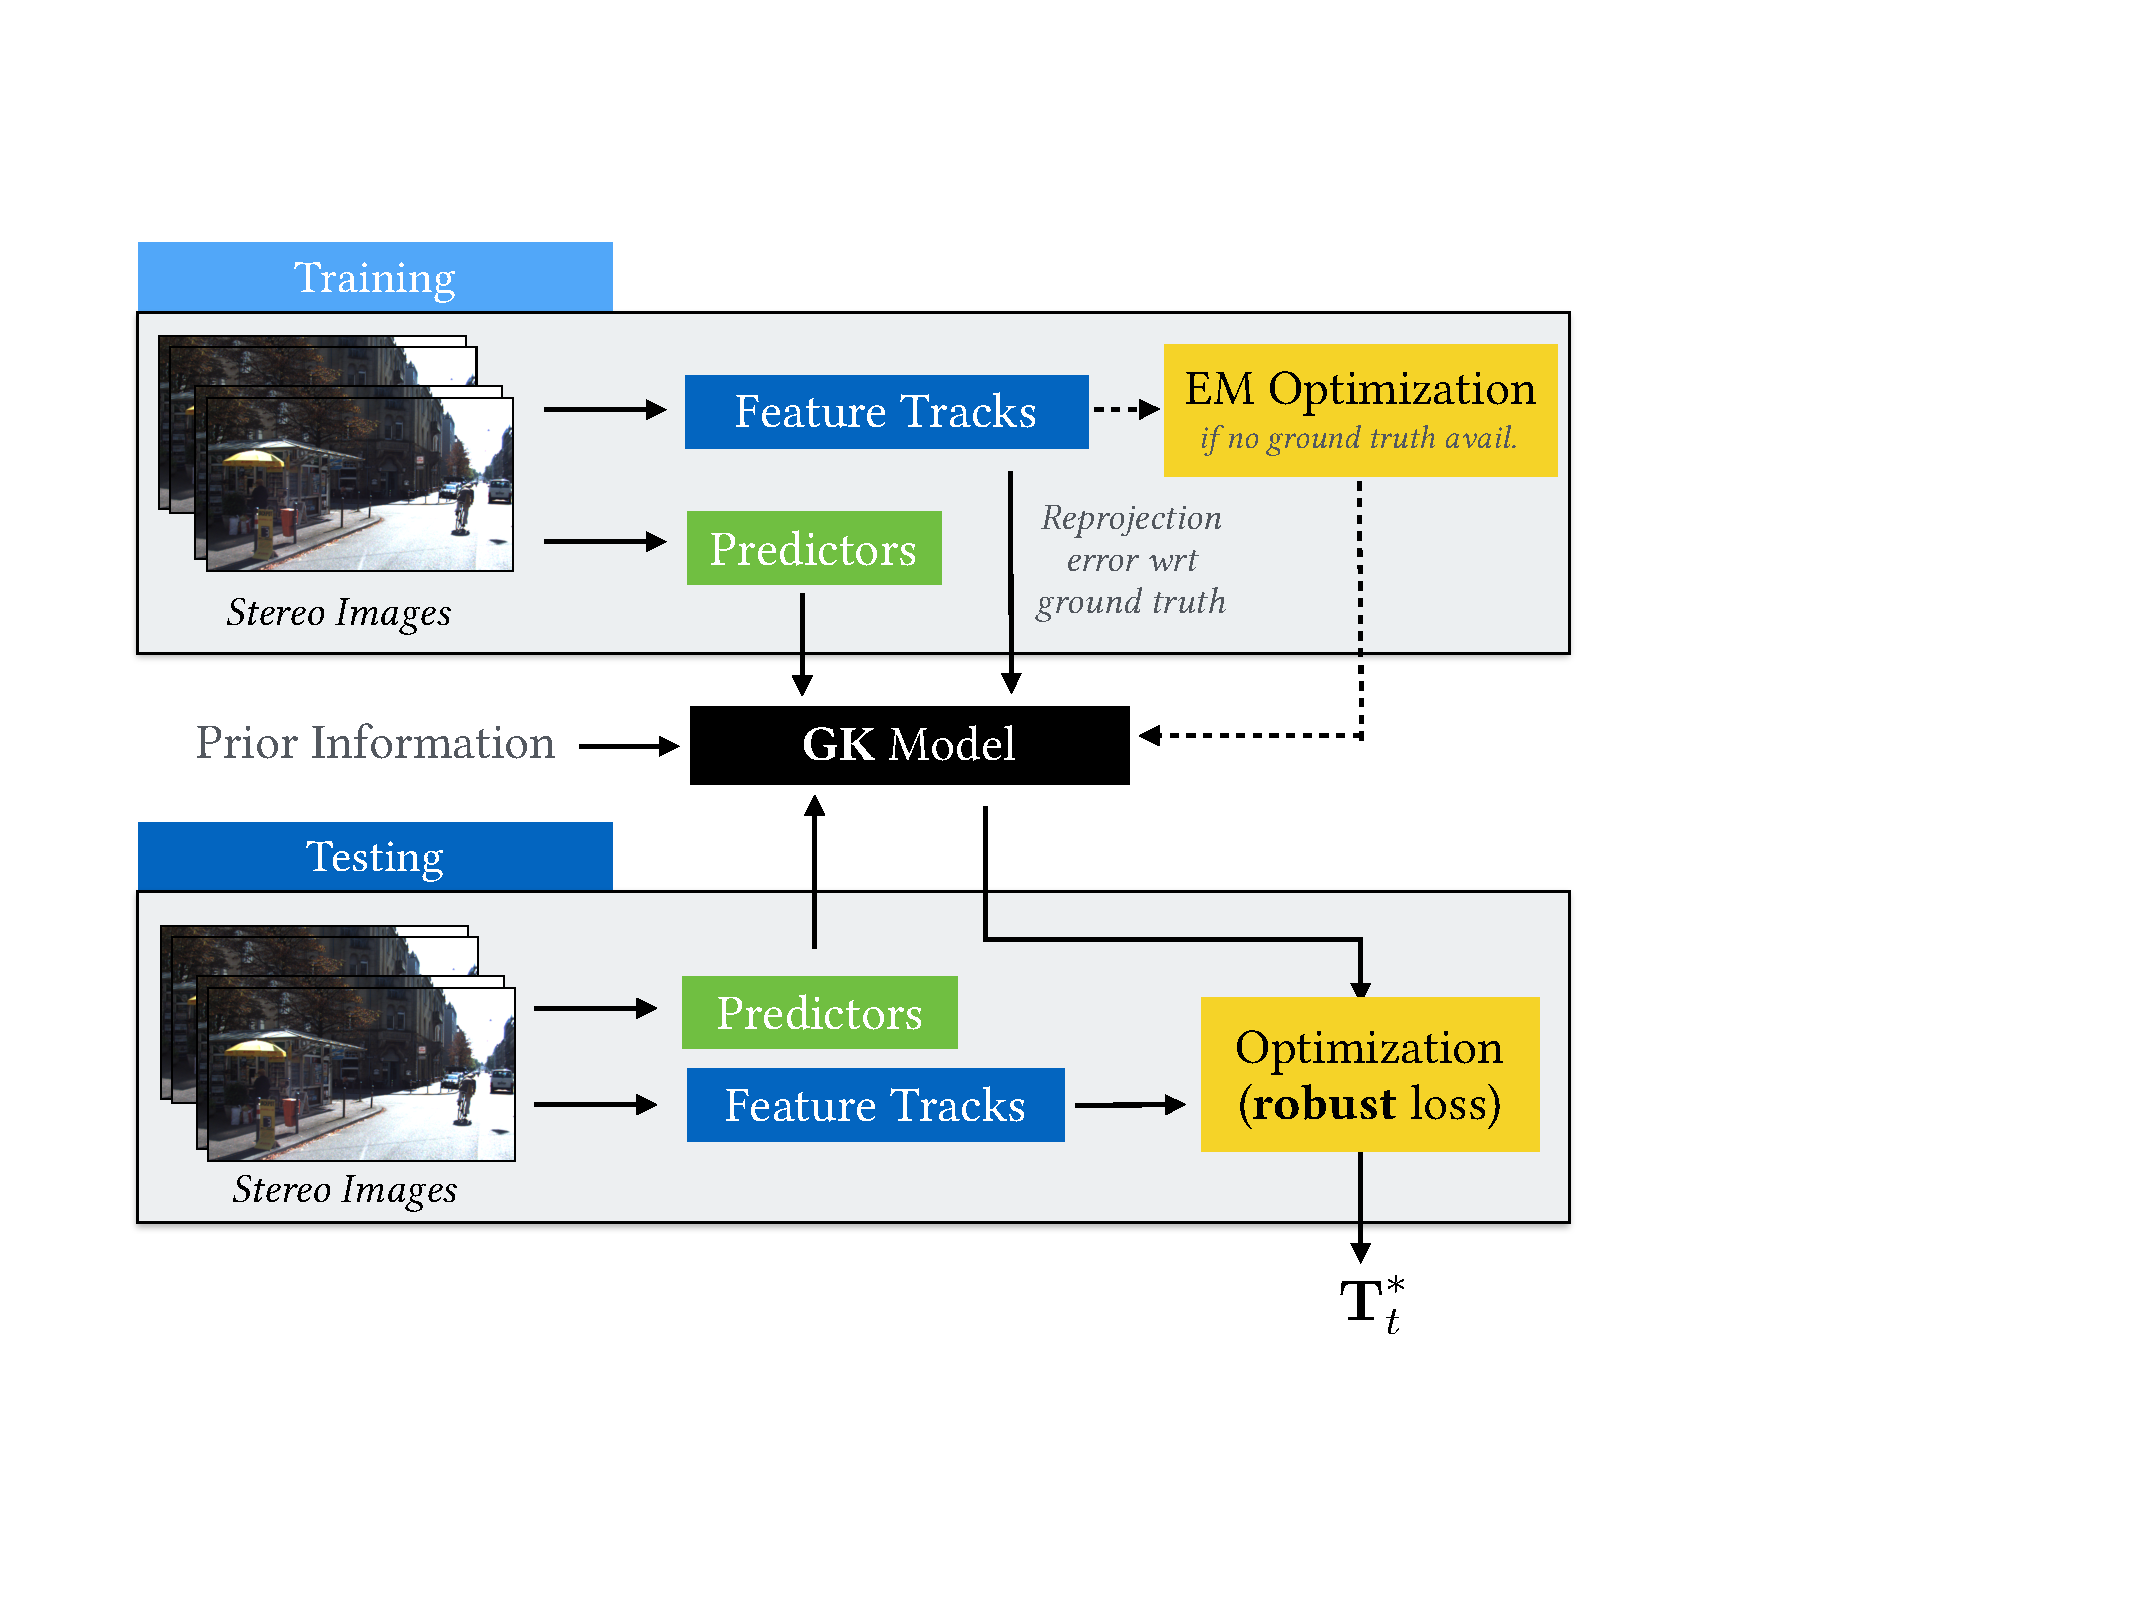
\includegraphics[width=\columnwidth]{sun-bcnn/system_overview}
      \caption{Our method uses a Bayesian Convolutional Neural Network (BCNN) to estimate the direction of the sun and to produce a principled uncertainty estimate for each prediction. We incorporate this \emph{virtual sun sensor} into a stereo visual odometry pipeline to reduce estimation error.}
    \label{fig:sun-bcnn_system}
\end{figure}

\begin{figure}
    \centering
    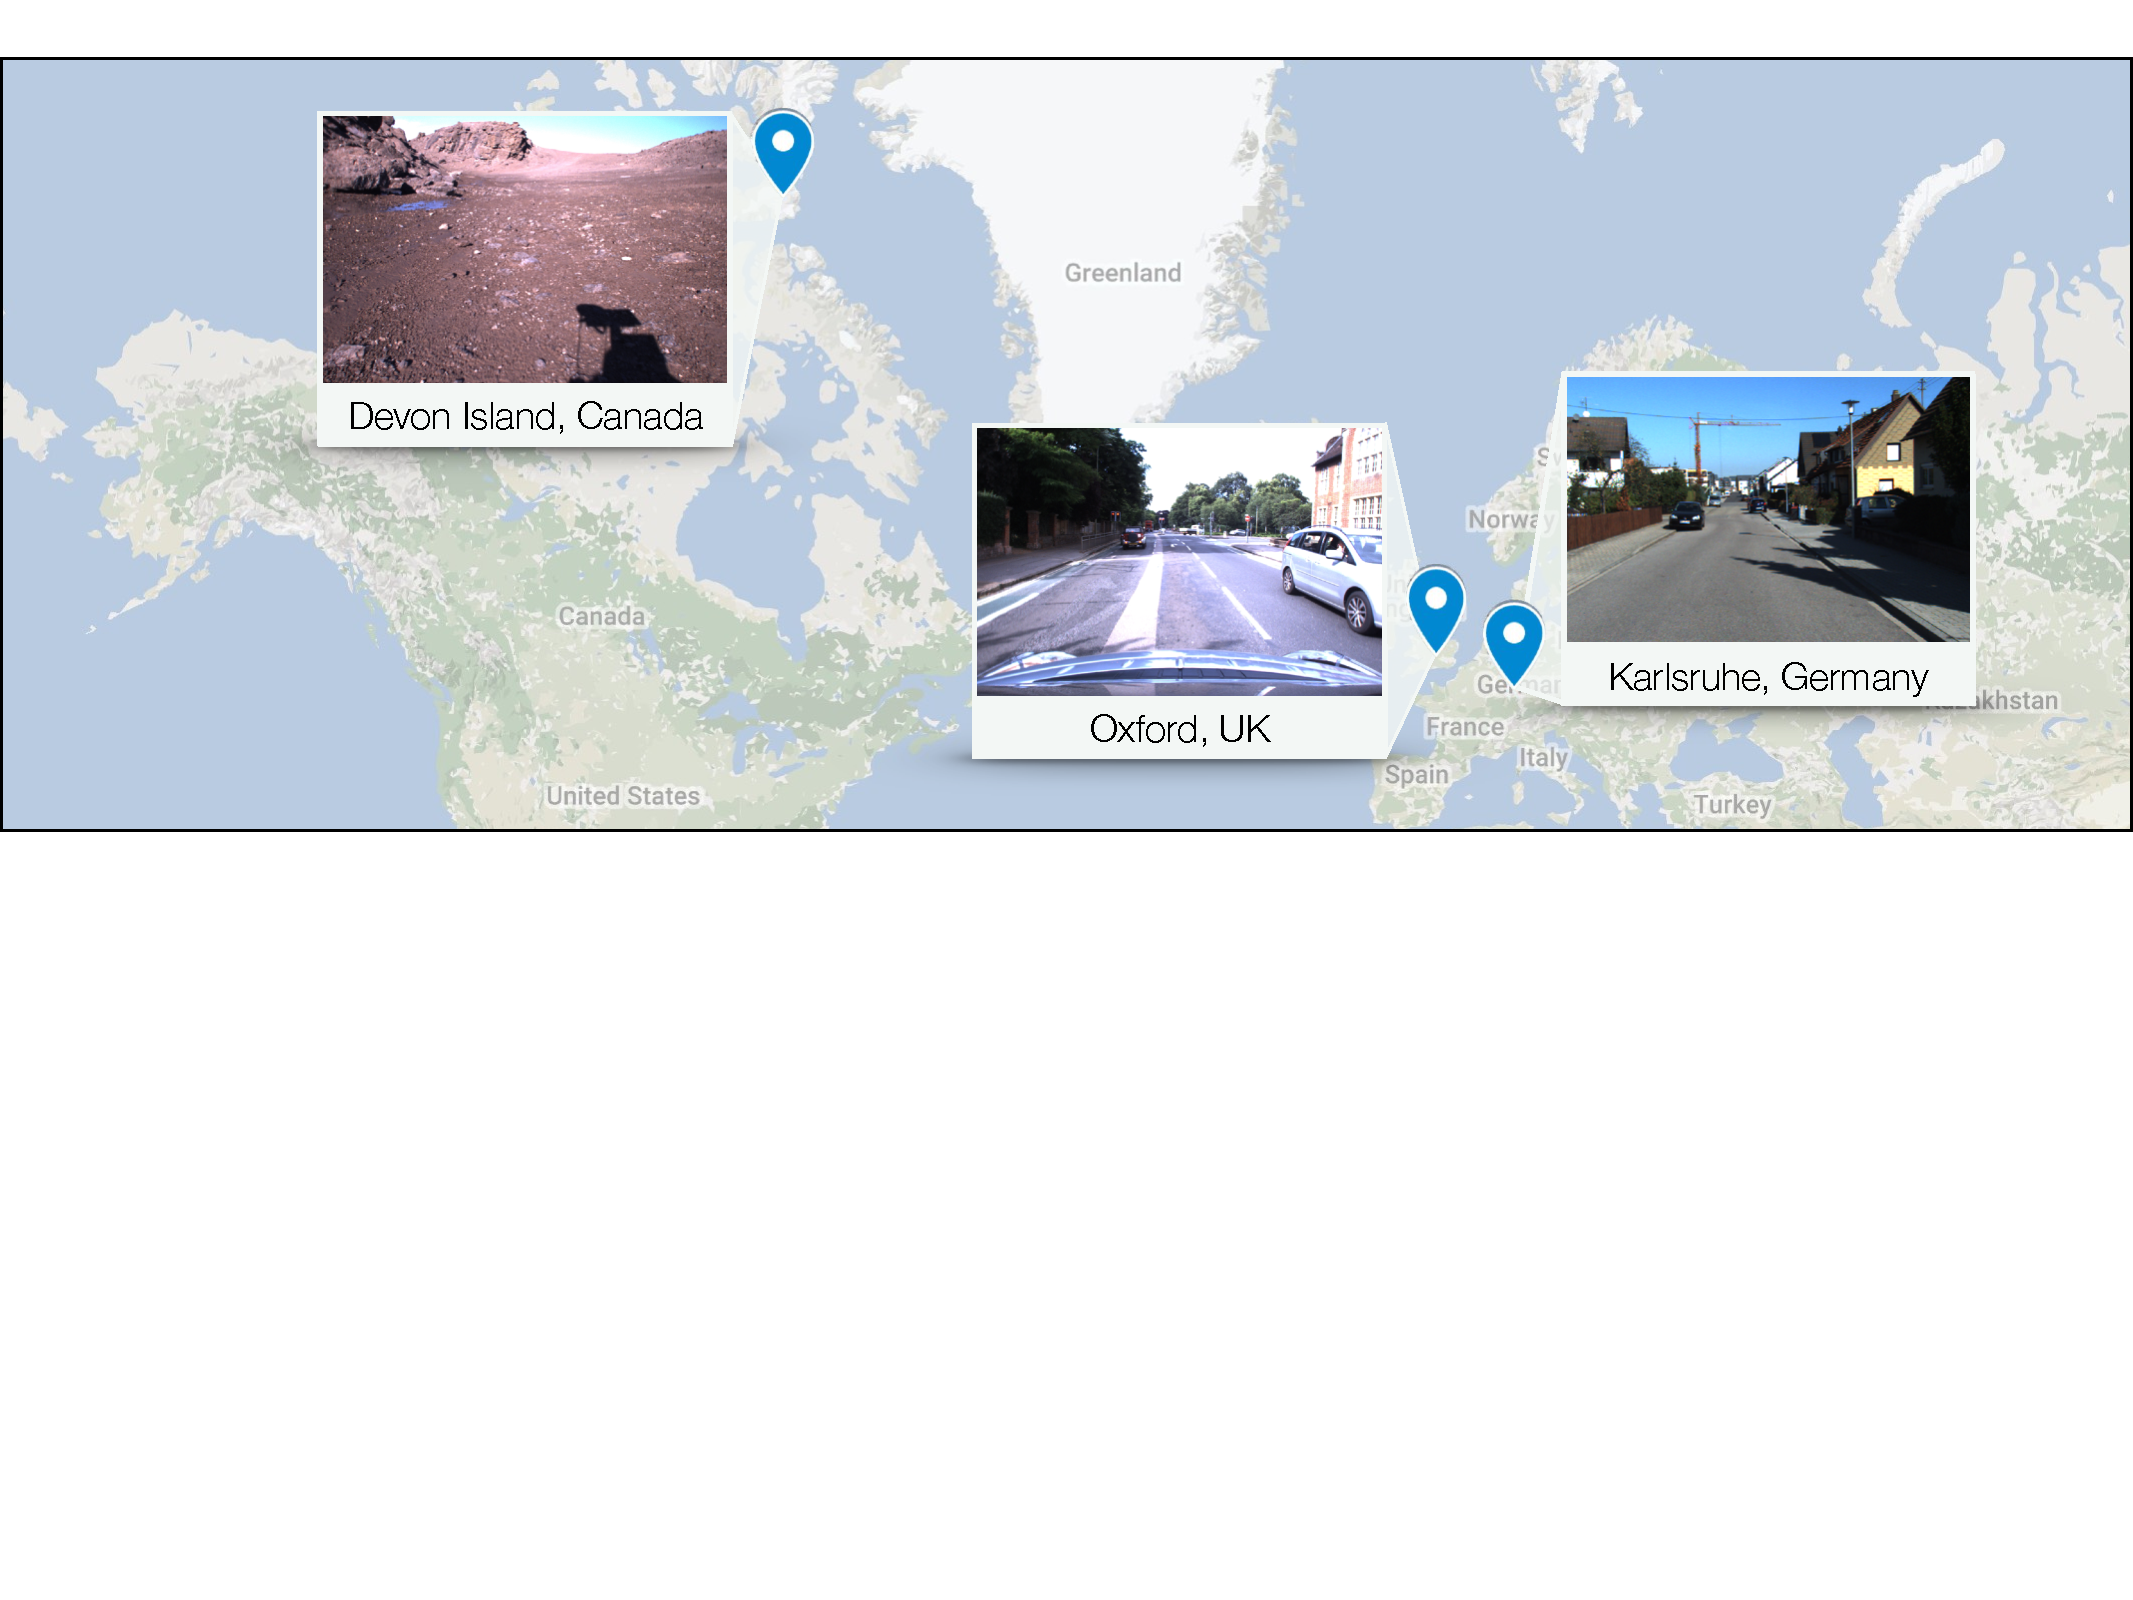
\includegraphics[width=0.98\textwidth]{sun-bcnn/all_datasets_gps}
    \caption{We train and test Sun-BCNN in a variety of environments ranging from urban driving in Europe to remote planetary analogue sites in the Canadian High Arctic. (Map data: Google, INEGI, ORION-ME.)}
    %\vspace{-0.4em}
    \label{fig:sun-bcnn_global-gps}
\end{figure}

For visual odometry (VO) in particular, the addition of global orientation information can limit the growth of drift error to be linear rather than superlinear with distance traveled \citep{Olson2003-ax}.
Sun-based orientation corrections have been successfully used in planetary analogue environments \citep{Furgale2011-zu,Lambert2012-um} as well as on board the Mars Exploration Rovers (MERs) \citep{Eisenman2002-cg,Maimone2007-tc}.
In particular, \citet{Lambert2012-um} showed that incorporating sun sensor and inclinometer measurements directly into the motion estimation pipeline (as opposed to periodically updating the vehicle heading, as in earlier work) can significantly reduce VO drift over long trajectories.

In this work, we seek to answer the question of whether similar reductions in VO drift can be obtained solely from the image stream already being used to compute VO.
The main idea here is that by reasoning over more than just the geometric information available from a standard RGB camera, we can improve existing VO techniques without needing to rely on a dedicated sun sensor or specially oriented camera.
In particular, we leverage recent advances in Bayesian Convolutional Neural Networks (BCNNs) to demonstrate how we can build and train a deep model capable of inferring the direction of the sun from a single RGB image. 
Moreover, we show that our network, dubbed Sun-BCNN, can produce a covariance estimate for each observation that obviates the need for a hand-tuned or empirically computed static covariance typically used for data fusion in a motion estimation pipeline. 

Our main contributions can be summarized as follows:
\begin{enumerate}
\item We apply a Bayesian CNN to the problem of sun direction estimation, incorporating the resulting covariance estimates into a visual odometry pipeline; 
\item We demonstrate that a Bayesian CNN with dropout layers after each convolutional and fully-connected layer can achieve state-of-the-art accuracy at test time;
\item We learn a 3D unit-length sun direction vector, appropriate for full 6-DOF pose estimation;
\item We present experimental results on over 30~km of visual navigation data in urban \citep{Geiger2012-fq} and planetary analogue \citep{Furgale2012-kk} environments; 
\item We investigate the sensitivity of our Bayesian CNN-based sun estimator (Sun-BCNN) to cloud cover, camera and environment changes, and measurement parameterization; and
\item We release Sun-BCNN as open-source \footnote{\url{https://github.com/utiasSTARS/sun-bcnn-vo}.}.
\end{enumerate}

The remainder of this paper begins with a discussion of related work, followed by an overview of the theory underlying BCNNs and a discussion of our model architecture, implementation, and training procedure.
We then outline our chosen visual odometry pipeline, which is based on a two-frame bundle adjustment optimization, and describe how observations of the sun can be incorporated directly into the motion estimation problem following the technique of \citet{Lambert2012-um}.
Finally, we present several sets of experiments designed to test and validate both Sun-BCNN and our sun-aided VO pipeline in variety of environments.
These include experiments on 21.6~km of urban driving data from the KITTI odometry benchmark training set \citep{Geiger2012-fq}, as well as a further 10~km traverse through a planetary analogue site taken from the Devon Island Rover Navigation Dataset collected in a planetary analogue site in the Canadian High Arctic \citep{Furgale2012-kk}.
We investigate the possibility of model generalization between different cameras and environments, and further explore the sensitivity of Sun-BCNN to cloud cover during training and testing, using data from the Oxford Robotcar Dataset \citep{Maddern2016-ng}.
We also examine the impact of different methods for computing the mean and covariance of a norm-constrained vector on the accuracy and consistency of the estimated sun directions.
